\begingroup
\setlength{\abovedisplayskip}{6pt}
\setlength{\belowdisplayskip}{6pt}
\setlength{\abovedisplayshortskip}{4pt}
\setlength{\belowdisplayshortskip}{4pt}
\setlength{\intextsep}{6pt}

\textbf{C.3.1. Model and assumptions.} Model the beam as a uniform, massless, linearly elastic cantilever with a lumped tip mass \(m\). Assume small horizontal deflection, one horizontal degree of freedom, no damping, and no applied horizontal force. The vertical support reaction balances the weight, so the horizontal vibration can be analyzed independently.

\textbf{C.3.2. Cross-sectional stiffness.} The beam bends in the horizontal direction shown in Figure 33. The cross-sectional dimension measured through the horizontal deflection direction is \(h\), while \(b\) is normal to that direction. Therefore, the relevant second moment of area is

\[
I=\frac{bh^3}{12}.
\]

Multiplying by the elastic modulus gives

\[
EI=E\frac{bh^3}{12}.
\]

\[
\boxed{I=\frac{bh^3}{12},
\qquad EI=\frac{Ebh^3}{12}}
\qquad\text{(C.3.2)}
\]

\textbf{C.3.3. Flex-beam spring constant.} For a concentrated load \(P\) at the free end of a cantilever, the maximum tip deflection is

\[
\Delta_{\max}=\frac{PL^3}{3EI}.
\]

The equivalent tip spring constant is the load divided by the tip deflection. Hence,

\[
k=\frac{P}{\Delta_{\max}}
 =\frac{3EI}{L^3}
 =\frac{3Ebh^3}{12L^3}.
\]

\[
\boxed{k=\frac{3EI}{L^3}}
\qquad\text{(C.3.3)}
\]

\textbf{C.3.4. Free-body diagram.} Take the horizontal displacement \(u(t)\) as positive to the right. The beam's equivalent spring force acts to the left and has magnitude \(ku\). The vertical support reaction \(N\) balances the downward weight \(mg\).

\begin{figure}[H]
\centering
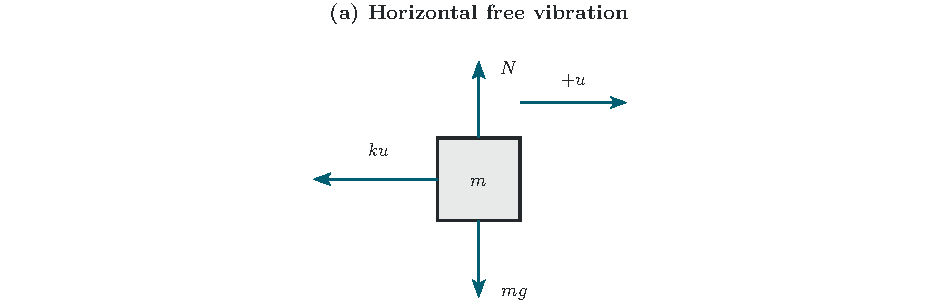
\includegraphics[width=0.95\linewidth,height=0.25\textheight,keepaspectratio,alt={Free-body diagram for horizontal flex-beam vibration in Problem C.3.}]{figures/generated/solutions/C3_fbd.pdf}
\caption{C.3.4. Free-body diagram for horizontal flex-beam vibration.}
\end{figure}

\textbf{C.3.5. Equation of motion.} The vertical forces balance because the mass has no vertical acceleration,

\[
\sum F_z=N-mg=0.
\]

In the horizontal direction, the spring reaction opposes the displacement, so

\[
\sum F_x=-ku(t).
\]

Applying Newton's law in the direction of motion gives

\[
m\ddot{u}(t)=\sum F_x=-ku(t).
\]

Rearranging produces the horizontal flex-beam equation of motion,

\[
\boxed{m\ddot{u}(t)+ku(t)=0}
\qquad\text{(C.3.5)}
\]

\textbf{C.3.6. Comparison with B.1.} The equation has the same form as the horizontal spring-mass equation in B.1. The difference is that the flex-beam stiffness is obtained from the cantilever relation \(k=3EI/L^3\), which gives

\[
\ddot{u}(t)+\frac{k}{m}u(t)=0,
\qquad
\omega_n=\sqrt{\frac{k}{m}}
 =\sqrt{\frac{3EI}{mL^3}}.
\]

Thus, the beam changes the value of \(k\) and \(\omega_n\), but not the form of the one-degree-of-freedom equation.

\[
\boxed{m\ddot{u}(t)+ku(t)=0,
\qquad \omega_n=\sqrt{\frac{3EI}{mL^3}}}
\qquad\text{(C.3.6)}
\]

\textbf{C.3.7. Initial value problem.} The undamped solution is written as

\[
u(t)=A\cos(\omega_nt)+B\sin(\omega_nt).
\]

Evaluating the displacement at \(t=0\) gives \(A=u_0\). Differentiating the response and evaluating the velocity at \(t=0\) gives \(\dot{u}_0=\omega_nB\), so \(B=\dot{u}_0/\omega_n\). Substitution gives the response for simultaneous initial displacement and initial velocity,

\[
\boxed{u(t)=u_0\cos(\omega_nt)
 +\frac{\dot{u}_0}{\omega_n}\sin(\omega_nt),
\qquad \omega_n=\sqrt{\frac{3EI}{mL^3}}}
\qquad\text{(C.3.7)}
\]

\endgroup
